\section{General Convex Optimization Solver}

I used cvxpy as the general convex optimization solver.

\section{Result}

Note: the result of cvxpy on the graph is that counted by cvxpy directly, which is independent of the number of rounds implemented in the Blahut-Arimoto algorithm.

\subsection{Symmetric Channel}

\subsubsection{Binary}

$P_{Y|X}=\matrix{1-p&p\\p&1-p}$ where $p=0.3$.\\
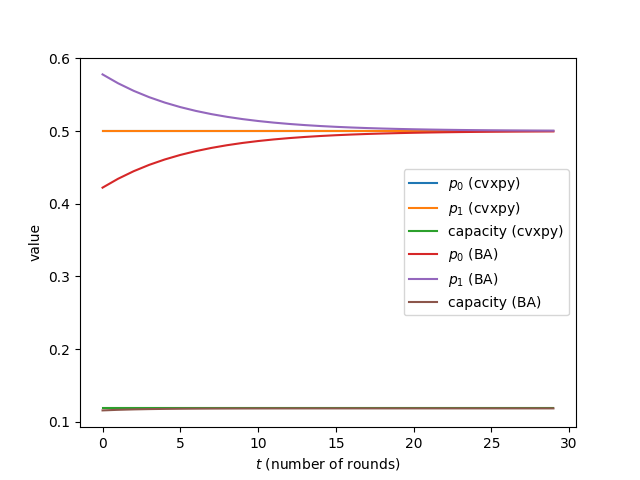
\includegraphics[width=15cm]{symmetric.png}\\
Result: uniform distribution.\\
Capacity: $\approx 0.119$.

\subsubsection{Complicated}

$P_{Y|X}=\matrix{
1-p&p/4&p/4&p/4&p/4\\
p/4&1-p&p/4&p/4&p/4\\
p/4&p/4&1-p&p/4&p/4\\
p/4&p/4&p/4&1-p&p/4\\
p/4&p/4&p/4&p/4&1-p
}$ where $p=0.3$.\\
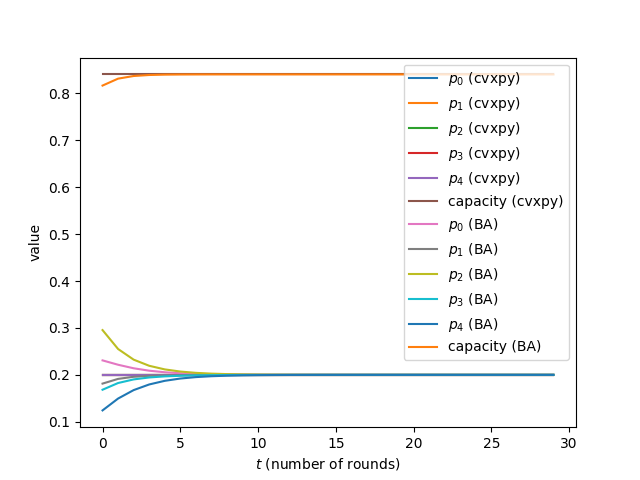
\includegraphics[width=15cm]{symmetric2.png}\\
Result: uniform distribution.\\
Capacity: $\approx 0.841$.

\subsection{Erasure Channel}

\subsubsection{Binary}

$P_{Y|X}=\matrix{1-p&p&0\\0&p&1-p}$ where $p=0.3$.\\
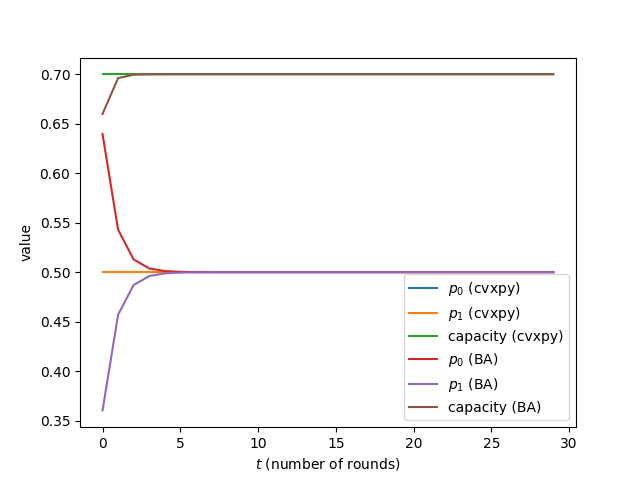
\includegraphics[width=15cm]{erasure.png}\\
Result: uniform distribution.\\
Capacity: $0.7$.

\subsubsection{Complicated}

$P_{Y|X}=\matrix{
1-p&0&0&0&0&p\\
0&1-p&0&0&0&p\\
0&0&1-p&0&0&p\\
0&0&0&1-p&0&p\\
0&0&0&0&1-p&p
}$ where $p=0.3$.\\
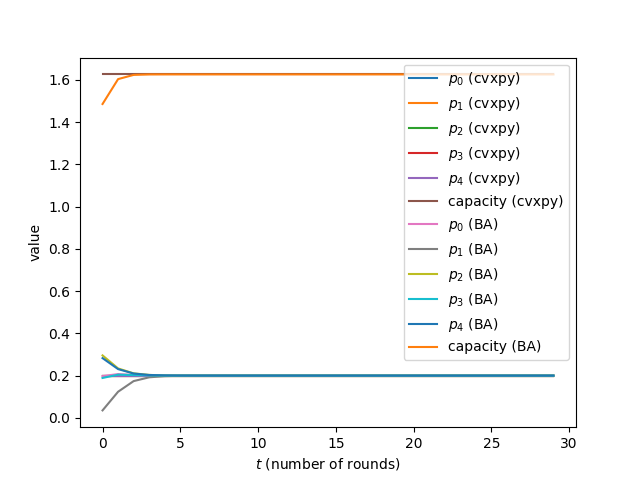
\includegraphics[width=15cm]{erasure2.png}\\
Result: uniform distribution.\\
Capacity: $\approx 1.625$.

\section{Source Code}

The following is my source code, where the \texttt{BA()} function is to compute the capacity by the Blahut-Arimoto algorithm, while the \texttt{general()} function is to compute using cvxpy.

\lstinputlisting{BA.py}

